% Supplemental Material for "Complex-contour regularization of second-order point-particle sources".
% DRAFT prepared with Claude Code, 16 October 2026. Numbers are from the Mathematica implementation
% in ../Mathematica implementation/ (stages 1-13; see README.md there).
\documentclass[aps,prl,onecolumn,superscriptaddress,nofootinbib,floatfix]{revtex4-2}
\usepackage{amsmath,amssymb}
\usepackage{graphicx}
\usepackage{bm}
\usepackage[colorlinks=true,linkcolor=blue!50!black,citecolor=blue!50!black,urlcolor=blue!50!black]{hyperref}
\usepackage{xcolor}
\graphicspath{{./}{../figures/prl/}{../figures/}}
\renewcommand{\Re}{\operatorname{Re}}
\renewcommand{\Im}{\operatorname{Im}}
\newcommand{\dext}{\delta_{\rm ext}}
\newcommand{\PhiP}{\Phi^{\rm P}}
\newcommand{\PhiS}{\Phi^{\rm S}}
\newcommand{\PhiR}{\Phi^{\rm R}}
\newcommand{\Pres}{\Phi^{\rm res}}
\newcommand{\x}{\mathbf{x}}
\newcommand{\Lop}{\mathcal{L}_\ell}
\renewcommand{\thefigure}{S\arabic{figure}}
\renewcommand{\thetable}{S\arabic{table}}
\renewcommand{\theequation}{S\arabic{equation}}

\begin{document}
\title{Supplemental Material: Complex-contour regularization of second-order point-particle sources}
\maketitle

\section{S1. Conventions and the linear-solve property}
Modes are $\Phi=\sum_\ell\phi_\ell(r)Y_{\ell0}(\theta)$, with $[f]_\ell=\sqrt{\pi(2\ell+1)}\int_{-1}^1 f\,P_\ell(\mu)\,d\mu$.
The first-order mode source is $\kappa_\ell\,\delta(r-r_0)$, with $\kappa_\ell=-(q/r_0^2)\sqrt{4\pi(2\ell+1)}$.
The ($\kappa_\ell=1$) Coulomb mode is $G_\ell=-r_0^2\,r_<^\ell/[(2\ell+1)r_>^{\ell+1}]$.

We use $H(z)=1+\tfrac{i}{\pi}\log(z-r_0)$ with the principal logarithm, and real-axis values are boundary values from above.
Logarithms of the form $\log[c(z-z_*)]$ are rewritten as $\ln|c|+\log(z-z_*)-i\pi[c<0]$.
This is the same function in the upper half-plane, and its principal value on the axis is the value from above.
Without this rewrite, Mathematica's $\log(r_0-r)$ at real $r>r_0$ lies on the wrong side of the cut.

\emph{Linear-solve property.}
$\Lop$ has real coefficients that are analytic away from $z=0$.
The solution continued along the contour therefore equals the boundary value from above of the solution in the region between the contour and the real segment.
Taking real parts commutes with $\Lop$.
So $\Re\tilde\psi(r+i0)$ solves $\Lop\psi=\Re\tilde s(r+i0)$ with the same real data at $a_L$.
Because $(\Delta r+i0)^{-n}=\mathrm{FP}\,\Delta r^{-n}+i\pi(-1)^n\delta^{(n-1)}(\Delta r)/(n-1)!$, the real part is the Hadamard finite part.

\section{S2. Consistency of the continued singular mode}
\emph{(i) Real part.}
Any solution $\psi$ of $\Lop\psi=\dext$ satisfies $\Re\psi(r+i0)-G_\ell=\alpha r^\ell+\beta r^{-\ell-1}$, because both sides solve the same real equation with the same $\delta$ source.
The singular structure at $r_0$ does not fix $\alpha$ and $\beta$; the 3D puncture does.

\texttt{DSolve}'s particular solution with constants set to zero gives the following ($\ell\le12$ checked):
\begin{itemize}
\item $\ell=0$: an anti-physical Green's function, $(\alpha,\beta)=(r_0,r_0^2)$;
\item $\ell=1$: the Coulomb mode;
\item $\ell\ge2$: a one-sided Green's function that vanishes for $r<r_0$, $\alpha=r_0^{1-\ell}/(2\ell+1)$.
\end{itemize}
Summed in 3D, these offsets give $-q/\rho+q\,r\cos\theta/r_0^2-q/r$ for $r<r_0$, and diverge for $r>r_0$.
If such a mode is used with 3D SS and SR, the computed second-order source is $Q[\Phi_1-\Delta,\Phi_1-\Delta]$ instead of $Q[\Phi_1,\Phi_1]$.

\emph{(ii) Imaginary part.}
Replacing $\Theta\to H$ in the Coulomb mode does not give a solution of $\Lop\psi=\dext$, because $\dext$ is not annihilated by smooth factors that vanish at $r_0$.
For $\ell=0$, $\mathcal L_0[-r_0+(r_0-r_0^2/z)H]=\dext-\tfrac{i}{\pi}z^{-1}$.
The residual field then acquires an $O(1)$ shadow, $r/(2\pi)$.
The fix is to add $\tfrac{i}{2\pi}z$.
Equivalently, use $\psi_p-D_\ell$, where $D_\ell$ is the homogeneous offset found in (i).

\section{S3. Shadow growth with truncated punctures}
With $\PhiP=q/\rho+cq\rho^n$ used consistently, the real-part mismatch vanishes identically.
The remaining contamination from products of continued modes is linear in $c$.
At fixed $\ell'_{\max}$ it falls by about $0.07$--$0.08$ per unit of $n$, but each coupled mode's contribution grows with $\ell'$.
Near $\ell'=30$ the growth per mode is $1.13$ and $1.19$ for $R=\tfrac12$, and $1.06$ and $1.09$ for $R=\tfrac14$, for the $Q=AB$ and $Q=\nabla A\cdot\nabla B$ toys respectively.
These are close to $1+R/r_0$ times a slowly varying power.

For fixed $R$ the total error therefore has a minimum in $\ell'_{\max}$.
Shrinking the worldtube as modes are added, $R=r_0/\ell'_{\max}$, keeps $(1+R/r_0)^{\ell'_{\max}}$ bounded, and the error then falls monotonically (Fig.~\ref{fig:lprime}).
For $Q=\tfrac12\partial_z^2(AB)$ the minimum lies near $\ell'_{\max}=12$--$16$ (main text, Fig.~4).
The hybrid split removes the contamination entirely.

\begin{figure}[h]
\centering
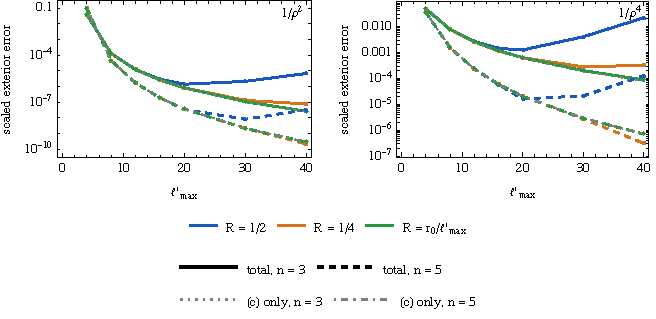
\includegraphics[width=0.75\textwidth]{fig_lprime_optimum.pdf}
\caption{Products of continued modes with a truncated puncture, for $Q=AB$ (left) and $Q=\nabla A\cdot\nabla B$ (right).
Exterior error against $\ell'_{\max}$ for $n=3$ (solid) and $n=5$ (dashed): fixed worldtubes $R=\tfrac12,\tfrac14$, and a shrinking worldtube $R=r_0/\ell'_{\max}$.
Dotted: mode-truncation error.}
\label{fig:lprime}
\end{figure}

\section{S4. Routes for continuing SS}
In the toy the SS modes are closed form, so they can be continued directly.
In GR they are available only from numerical angular quadrature.
We compared three ways of putting them on the contour, treating the toy data as if numerical (Fig.~\ref{fig:ssreuse}).
\begin{itemize}
\item \emph{Route 2 (hybrid).} Subtract the analytic singular terms and Cauchy-continue the real-axis remainder.
  Subtracting only $A_\ell/\Delta r^2$, or $A_\ell/\Delta r^2+B_\ell/\Delta r$, fails ($0.4$ and $0.3$ at grid spacing $h=0.005$), because the remaining $\ln|\Delta r|$ cannot be interpolated.
  Including $C_\ell\ln|\Delta r|$ gives $O(h^3)$ ($3\times10^{-7}$), and the next two log terms give $O(h^5)$ ($3\times10^{-12}$).
  However, $10^{-8}$ relative noise on the SS samples produces an error of $7\times10^{-4}$: subtracting $A_\ell/\Delta r^2$ amplifies the noise by $10^4$--$10^5$.
\item \emph{Radial factor.} Continue $F_\ell=(r-r_0)^2\mathrm{SS}_\ell$, which is bounded, and divide by $(z-r_0)^2$ on the contour.
  The shadow of $F$ at $r_0$ must be pinned to remove spurious $\delta'$ and $\delta$ terms. Without pinning the error is $23$, matching the predicted $-\pi G_0\delta'+\pi G_1\delta$ to $10^{-14}$.
  With exact pinning constants the error is $O(h^3)$. With constants taken from the data, $G_1$ is wrong by $O(h\ln h)$, because of the $\Delta r^2\ln|\Delta r|$ term in $F$, and the method is only first order.
\item \emph{Route 1 (complex-$r$ quadrature).} Evaluate $\mathrm{SS}_\ell(z)=\oint Q[\PhiP,\PhiP](z,\theta)\,Y_{\ell0}\,d\Omega$ directly at the contour nodes.
  The integrand is smooth except near the crossing of $|z|=r_0$, where the angular path is deformed.
  The result agrees with the closed-form continuation to $1.8\times10^{-14}$ on the contour and $1.7\times10^{-12}$ in the exterior, at a cost similar to real-axis quadrature near $r_0$.
  No singular quantity is subtracted.
\end{itemize}
Route 1 also works for SR Part 1 ($10^{-13}$), and for the full SR with an exact puncture ($4\times10^{-14}$).
For pieces whose modes have kinks at $r_0$, the angular integral at complex $r$ gives a single analytic branch.
The inside and outside branches of the \emph{undifferentiated} products must therefore be blended with $H$ before $\partial_z^2$ is applied. Blending the finished source instead fails (errors $3$--$900$).

Summing continued residual modes at complex $r$, $\sum_{\ell'}\tilde\phi^{\rm res}_{\ell'}(z)Y_{\ell'0}(\theta)$, is asymptotically divergent for truncated punctures: terms grow by $1.05$--$1.07$ per $\ell'$ beyond $\ell'\approx30$.
This is why SR Part 2 is formed on the real axis.

\begin{figure}[h]
\centering
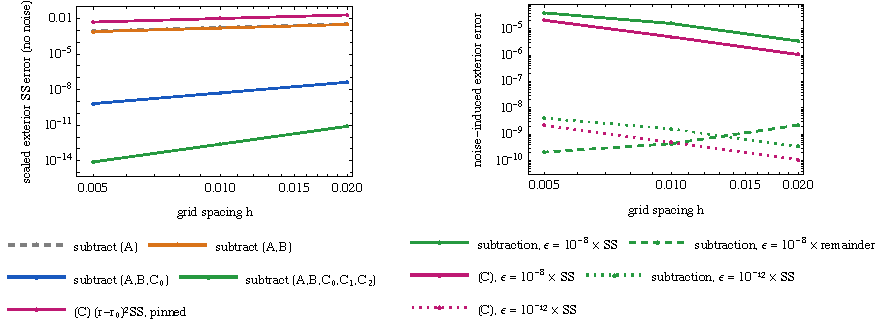
\includegraphics[width=0.85\textwidth]{fig_ss_reuse.pdf}
\caption{Continuing SS from data treated as numerical. Left: error against grid spacing for the subtraction variants and the pinned radial factor. Right: noise propagation.}
\label{fig:ssreuse}
\end{figure}

\section{S5. Convergence of the hybrid split}
With $\PhiP=q/\rho+cq\rho^n$, the residual $\PhiR-cq\rho^n$ is $C^{n-1}$ at $\x_0$.
Its coupled-mode contributions fall as $\ell'^{-(n+3)}$, so the truncation error falls as $\ell'^{-(n+2)}_{\max}$.
The fitted slopes are $2.99$, $4.95$, $6.91$ and $8.87$ for $n=1$, 3, 5 and 7 (Fig.~\ref{fig:conv}).
Inside $r_0$ the error is largest next to the worldtube. Outside, it grows towards $r=10$, because the Cauchy data are set at $r=1$.

Fitting the large-$\ell'$ tail with two terms of the $\Lambda_{\ell,s,n}$ functions of Refs.~\cite{Upton2026S,HOW2012S} gains a factor of 38--113 at $\ell'_{\max}=20$ and up to $2000$ at $\ell'_{\max}=30$.
At $\ell'_{\max}=12$ the two-term fit makes the error worse; a one-term fit gains a factor of about 1.5 there.
The hybrid split adds no error of its own: the Cauchy step contributes below $10^{-14}$, and the split reproduces the mode-truncation error to better than $10^{-6}$ relative.

\begin{figure}[h]
\centering
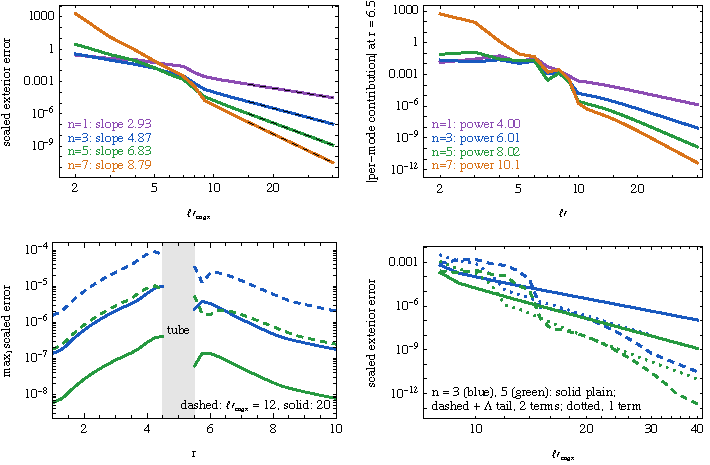
\includegraphics[width=0.85\textwidth]{fig_hybrid_convergence.pdf}
\caption{Hybrid split, $Q=\tfrac12\partial_z^2(AB)$, $k=0$.
Top: error against $\ell'_{\max}$ with fitted slopes, and per-mode contributions against $\ell'$.
Bottom left: error against $r$.
Bottom right: tail acceleration.}
\label{fig:conv}
\end{figure}

\section{S6. Comparison with Musaeus, Pound and Upton}
\emph{Mode-level finite part.}
For the operator $r^2\partial_r^2-2r\partial_r-(\ell-1)(\ell+2)$ with the Green's function of their Eq.~140, and sources $A/\Delta r^4+B/\Delta r^3+C/\Delta r^2+D/\Delta r$, we compared three calculations for $\ell=2$--$6$:
\begin{itemize}
\item their prescription (Eqs.~141 and A2--A5);
\item an independent Taylor-subtracted finite part, which agrees with it to below $10^{-38}$, independently of the cutoff;
\item the contour integral $\Re\int_CG\,S\,dz$, which agrees with both to $4\times10^{-34}$ for five choices of worldtube radius and contour height.
\end{itemize}
Their closed form, Eq.~142, is confirmed.

\emph{$T_Q$ and the mode-level $\delta$ content} (exact puncture, $Q=\tfrac12\partial_z^2(AB)$).
The canonical SR is $q\,\partial_z^2(\PhiR/\rho)$, a derivative of an integrable function.
Its 4D finite part is the ball-excluded principal value, and the difference between the two is $T_Q=-\tfrac{4\pi}{3}q\PhiR(\x_0)\delta^3$, verified to $10^{-21}$.

At mode level, the total $\delta$ coefficient is $c_\ell=-4\pi q\PhiR(\x_0)Y_{\ell0}(0)/r_0^2$. It splits as $\tfrac23c_\ell$ from the finite part plus $\tfrac13c_\ell$ from $T_Q$.
Scaled exterior errors for each prescription:
\begin{center}
\begin{tabular}{lc}
\hline\hline
prescription & error ($\ell\le6$)\\
\hline
contour, canonical source & $<10^{-27}$\\
modes of the 4D finite part $+\;T_Q$ (their Eq.~24) & $<10^{-17}$\\
modes of the 4D finite part, without $T_Q$ & $0.14$--$170$\\
pointwise modes, mode-level finite part (their Eq.~105) $+\;T_Q$ & $0.27$--$340$\\
pointwise modes, no $\delta$ terms & $0.41$--$500$\\
\hline\hline
\end{tabular}
\end{center}
The shell (mode-level) and ball (4D) regulators do not commute for the trace-free $\rho^{-3}$ term: a term proportional to $B'/(B+B')$ survives.

\section{S7. Numerical details}
All computations use working precision 30 and exact rational parameters.
NDSolve is run with PrecisionGoal 20, AccuracyGoal 35 and \texttt{InterpolationOrder -> All}.
Contour sources are evaluated at numerical $y(a)$. Symbolic composition expands them into high-degree polynomials and loses all accuracy.

The Cauchy step uses Gauss quadrature after subtracting the cubic Taylor polynomial of $s$ about $\Re z$, which is integrated analytically. The source on the contour is represented piecewise at 40-digit precision.

The full test suite has more than 2,000 automated checks.

\begin{thebibliography}{9}
\bibitem{Upton2026S}
S.~D.~Upton, B.~Wardell, A.~Pound, N.~Warburton, and L.~Barack, arXiv:2508.00087 [gr-qc] (2026).
\bibitem{HOW2012S}
A.~Heffernan, A.~Ottewill, and B.~Wardell, Phys.\ Rev.\ D \textbf{86}, 104023 (2012).
\end{thebibliography}

\end{document}
